\documentclass{book} 

\usepackage{indentfirst}
\usepackage{booktabs}
\usepackage{multirow}
\usepackage{framed}
\usepackage{graphicx}
\usepackage{float}
\begin{document}
\title{Final Project Report}
\author{Zhou Litao, Fang Shaoheng, Dong Shiwen, Yang Hongbo}
\date{\today}




\maketitle


\tableofcontents



\frontmatter

\chapter {Preface}

\section* {Who we are}

We are a group of freshman students at SJTU working for the 2019 Spring EE101 course final project. We are heading for a website which allows users to search for papers and learn more about the details from our webpage and visualized charts. Our website is a local one based on a local MySQL database and a local solr search engine. The programming and coding languages we've used in this project involves Python, PHP, javascript, HTML and CSS.

\section* {What we have}

Start from the index page, by typing the keywords you want to search about, you can access the search page. And then you can jump between all the information pages as you will. 

Based on the type of data and the way we present them, the contents of our web fall into 5 parts, namely search (result), papers, authors, affiliations and conferences. Every section is made up of several subpages demonstrating different functions. The main functions and features of every section are listed as follows. The name behind every row represents the person who mainly takes charge, but it should be decleared that all the team members have been helping address each other's probelms all the way through the project, and must have somehow contributed to the part that he is not in charge of.

\begin{figure}[H]
\centering
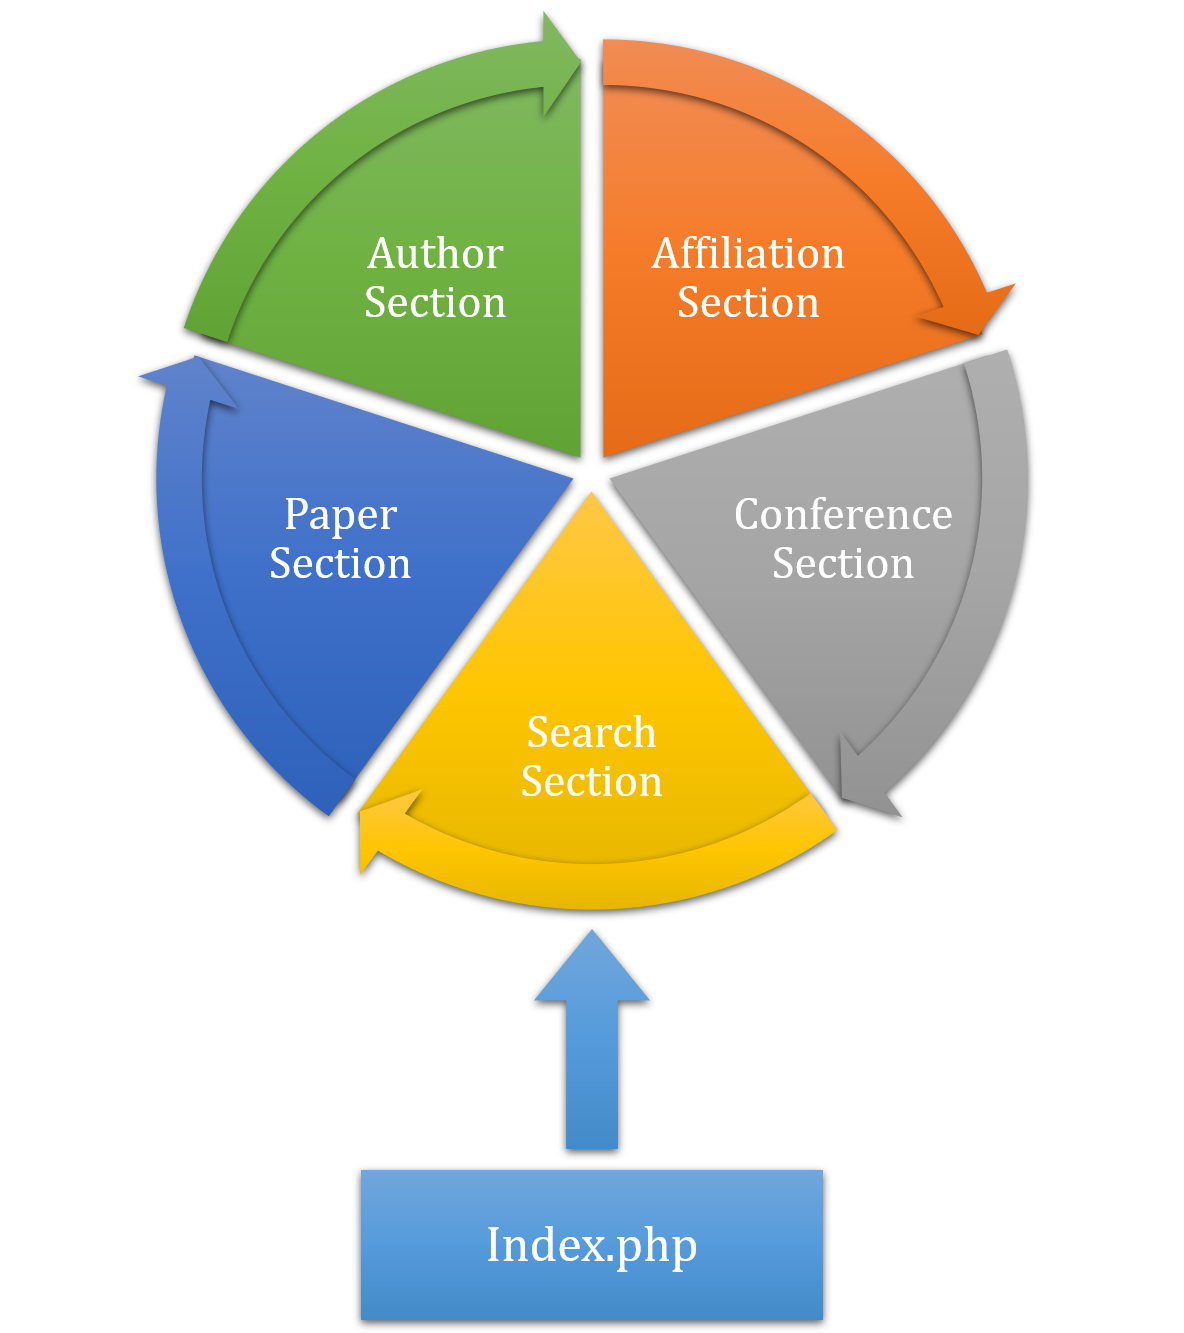
\includegraphics[scale=0.5]{img/zlt_pre_1.png}
\caption{General Structure of our Web}
\end{figure}

\paragraph{index.php}

\begin{itemize}
\item An Integrated Search Bar \textit{by Shaoheng Fang}
\item A 3D-Graph Showing the Distribution of Years and Conferences \textit{by Shaoheng Fang}
\item The Transplantation \& modification of an online Template  \textit{by Shaoheng Fang}
\end{itemize}

\paragraph{Search Section}
\begin{itemize}
\item Search Results Formatting \textit{by Litao Zhou}
\item Visulized Graphs \textit{by Shaoheng Fang}
\begin{itemize}
	\item Publish Year
	\item Conference
	\item Top Authors
\end{itemize}
\item Leaf Flipping in Search Results \textit{by Shiwen Dong}
\end{itemize}

\paragraph{Paper Section}
\begin{itemize}
\item Paper Information \textit{by Litao Zhou}
\item Paper Relation Chart \textit{by Litao Zhou}
\item Leaf Flipping in multiple Pages \textit{by Shiwen Dong}
\item Paper Reference/Citations/Recommendation  \textit{by Hongbo Yang}
\end{itemize}

\paragraph{Author Section}
\begin{itemize}
\item Author Information \textit{by Litao Zhou}
\item Visulized Graphs \textit{by Shaoheng Fang}
\begin{itemize}
	\item Publish Year (Pie Chart \& Bar Chart)
	\item Conference (Pie Chart \& Bar Chart)
\end{itemize}
\item Leaf Flipping in Author Publications \textit{by Shiwen Dong}
\end{itemize}

\paragraph{Affiliation Section}
\begin{itemize}
\item Affiliation Author List \& Conference List \textit{by Litao Zhou}
\item Visulized Graphs \textit{by Shaoheng Fang}
\begin{itemize}
	\item Publish Year
	\item Top Author by Reference
	\item Top Author by Publication
\end{itemize}
\item Leaf Flipping in Author List and Conference List \textit{by Shiwen Dong}
\end{itemize}

\paragraph{Conference Section}
\begin{itemize}
\item Paper Table \textit{by Litao Zhou}
\item Paper Publish Year Graph \textit{by Shaoheng Fang}
\item Author Relation Big Graph by Gephi \textit{by Hongbo Yang}
\item Leaf Flipping in Paper Table \textit{by Shiwen Dong}
\end{itemize}


\section* {How we work together}

The making of a website requires frequent communication of source codes. In response, we use Github as a platform to exchange our codes. At the beginning of our project, we took some time to learn how Git works and created a uniform database and solr engine to make our codes work on everyone's computer. Then every member will be working and making progress on his own branch. We can use the Git system to merge our progress onto the master branch when necessary, and distribute the new version to everyone's branch. With the help of the Git system, we no longer have to bother comparing different codes written by multiple collaborators or having trouble with the inconsistency in others' codes. The network graph was derived from our Github repository homepage, where our commits and branches are displayed.

\begin{figure}[H]
\centering
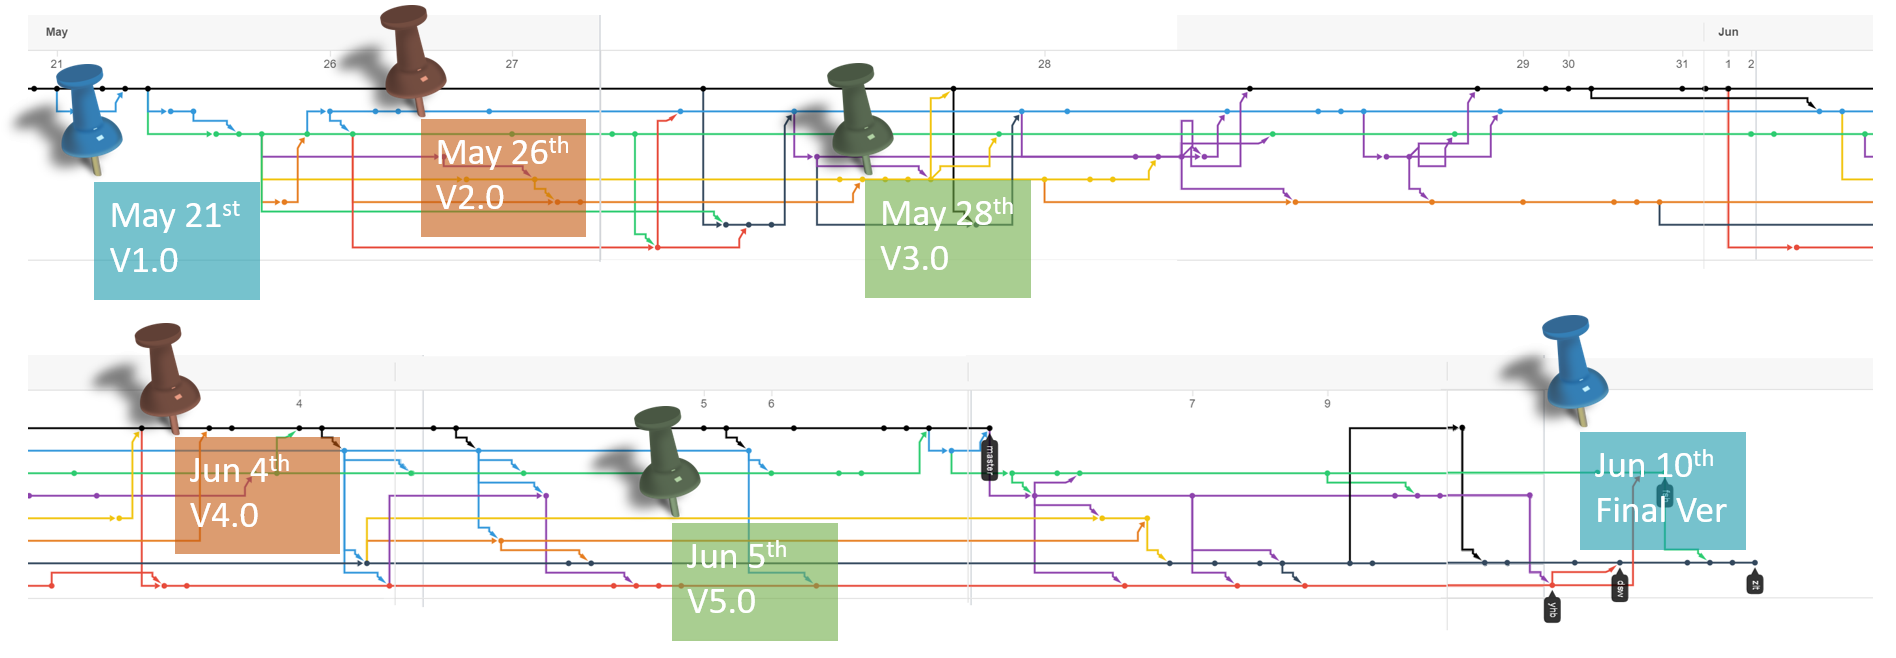
\includegraphics[scale=0.25]{img/zlt_pre_2.png}
\caption{Our Developing Story}
\end{figure}

\section* {How to Check our Work}

To see our source codes, you can visit our github repository homepage (https://github.com/ltzone/EE101Lab) and clone our repository. You can also see the LaTeX source codes in the report folder. In order to make our website work on your computer, you have to follow our guide in the configguide.txt. This guide will help you initialize your MySQL database and Solr engine and write all the information into them. You may also check our presentation slides to see the detail of our developing story.



\mainmatter
\chapter {Enrich the Contents}

\section {Paper \& Conference Pages}

These parts are requred as a necessary part of final lab. We want to display useful information to users. So we added functions to search for more detailed relavant messages.
Depending on the characteristics of each field, we used different methods to show information.


\subsection{Description}

\subsection{Solution}

\paragraph{point 1}

\paragraph{point 2}

\subsection{Source Codes}

\begin{minipage}[r]{15em}
\begin{verbatim}

short code example

\end{verbatim}
\end{minipage}

\subsection{Explanation}

\subsection{Demonstration}

\begin{figure}[H]
\centering

\includegraphics[height=4.0cm,width=4.0cm]{img/yhb_1.jpg}
\caption{IMG EXAMPLE}
\end{figure}

\section {Affiliation Pages}

We'd like to add a new series of pages to show affiliation information to users. Since we didn't do any previous work about affiliation information in the previous labs except that the affiliation table was input into the database, we have to write new SQL commands in search of affiliation information, and echo them out on the pages. The paper table and charts on other pages can be of help in showing the affiliation related information. Also, we have already got the author table written in the paper information page. Generally speaking, the work here is to collect the affiliation data and arrange them in order on the pages.


\subsection {General Description}

The final version of the affiliation section include 3 concrete pages. On the affiliation\_info.php page, we will give three numbers on top of the page, counting all the authors, papers, and references in the affiliation. Then the authors in the affiliation will be listed below, together with their own affiliation information (hyper-links included) and number of publications. Affiliation\_paper.php shows all the papers related to the affiliation. The affiliation\_charts.php, where three charts are displayed, will be reported in detail in the Statistical Graph Section.

\begin{figure}[H]
\centering
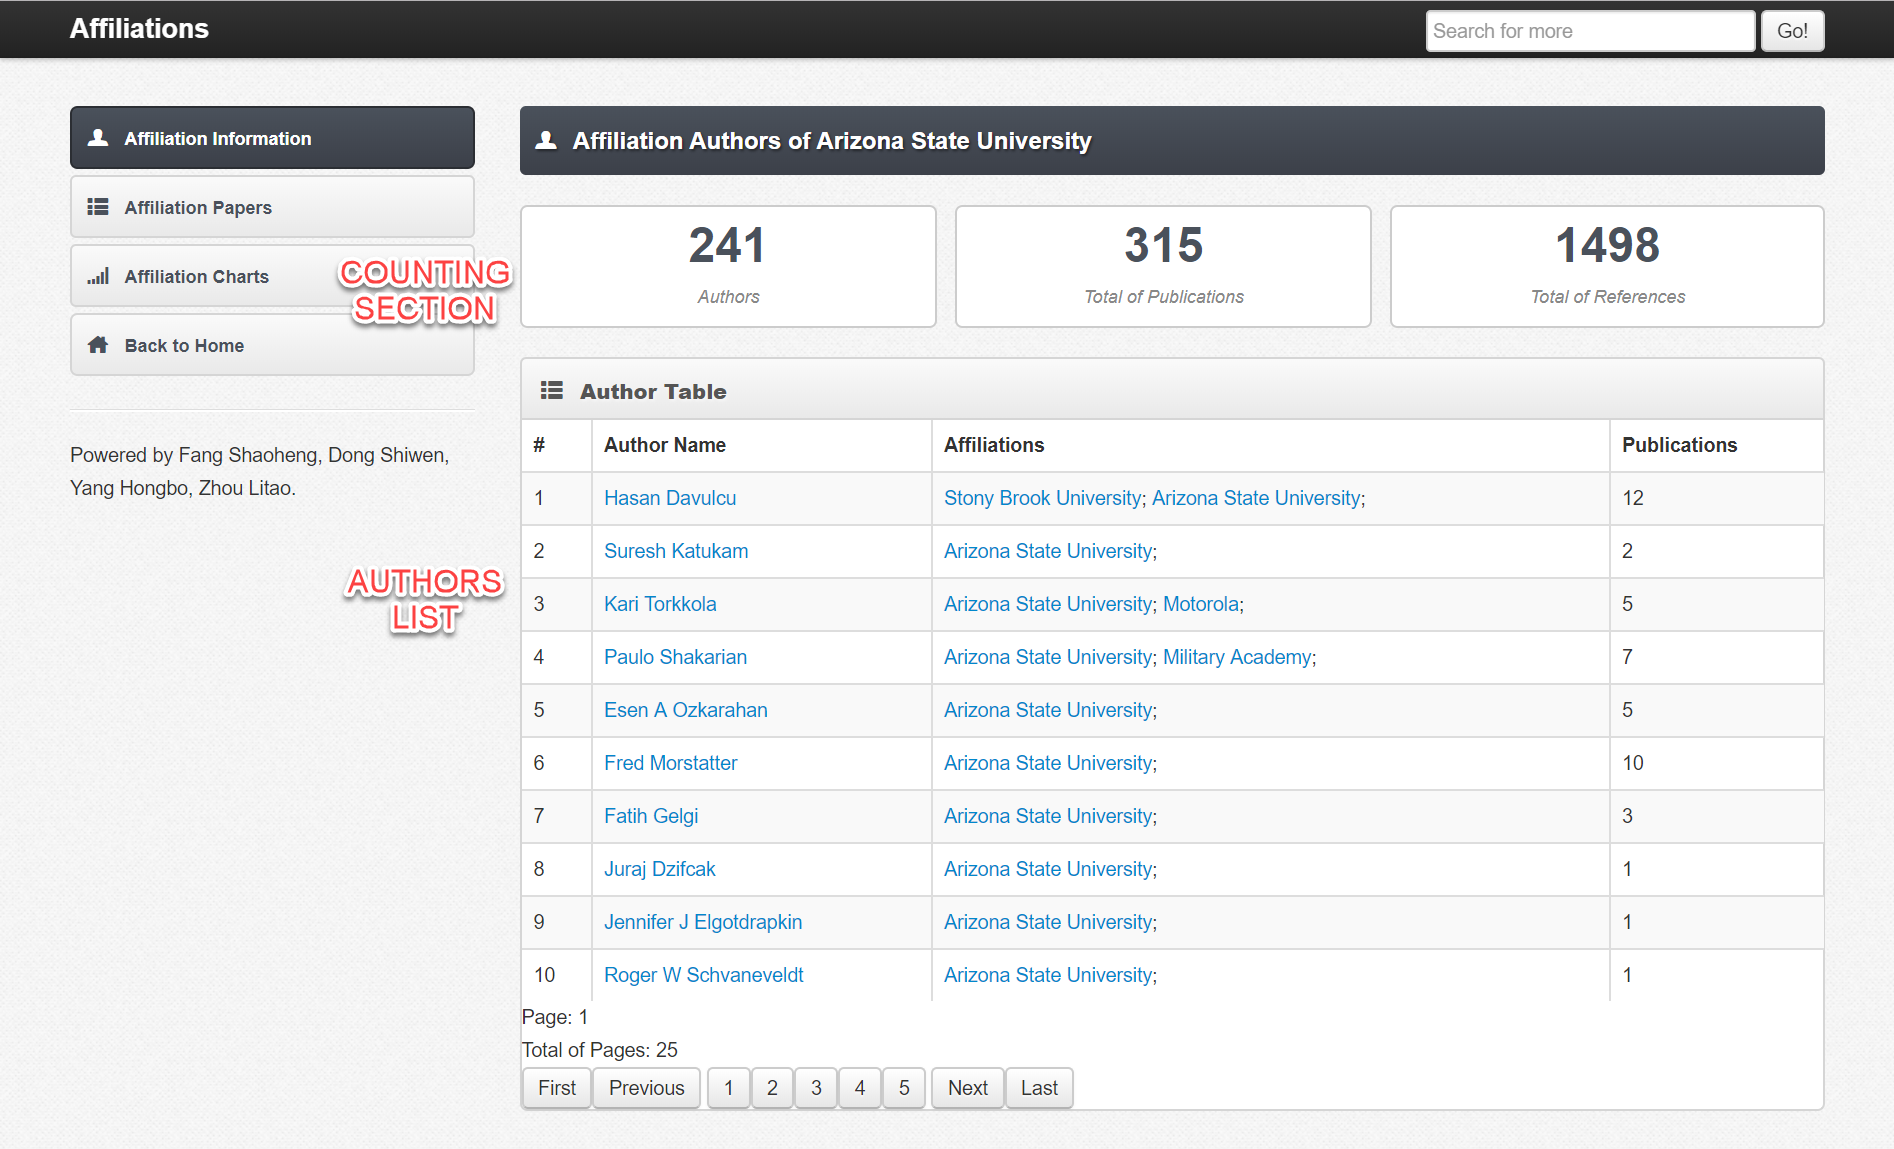
\includegraphics[scale=0.35]{img/zlt_aff_demo1.png}
\caption{affiliation\_info.php page}
\end{figure}

\begin{figure}[H]
\centering
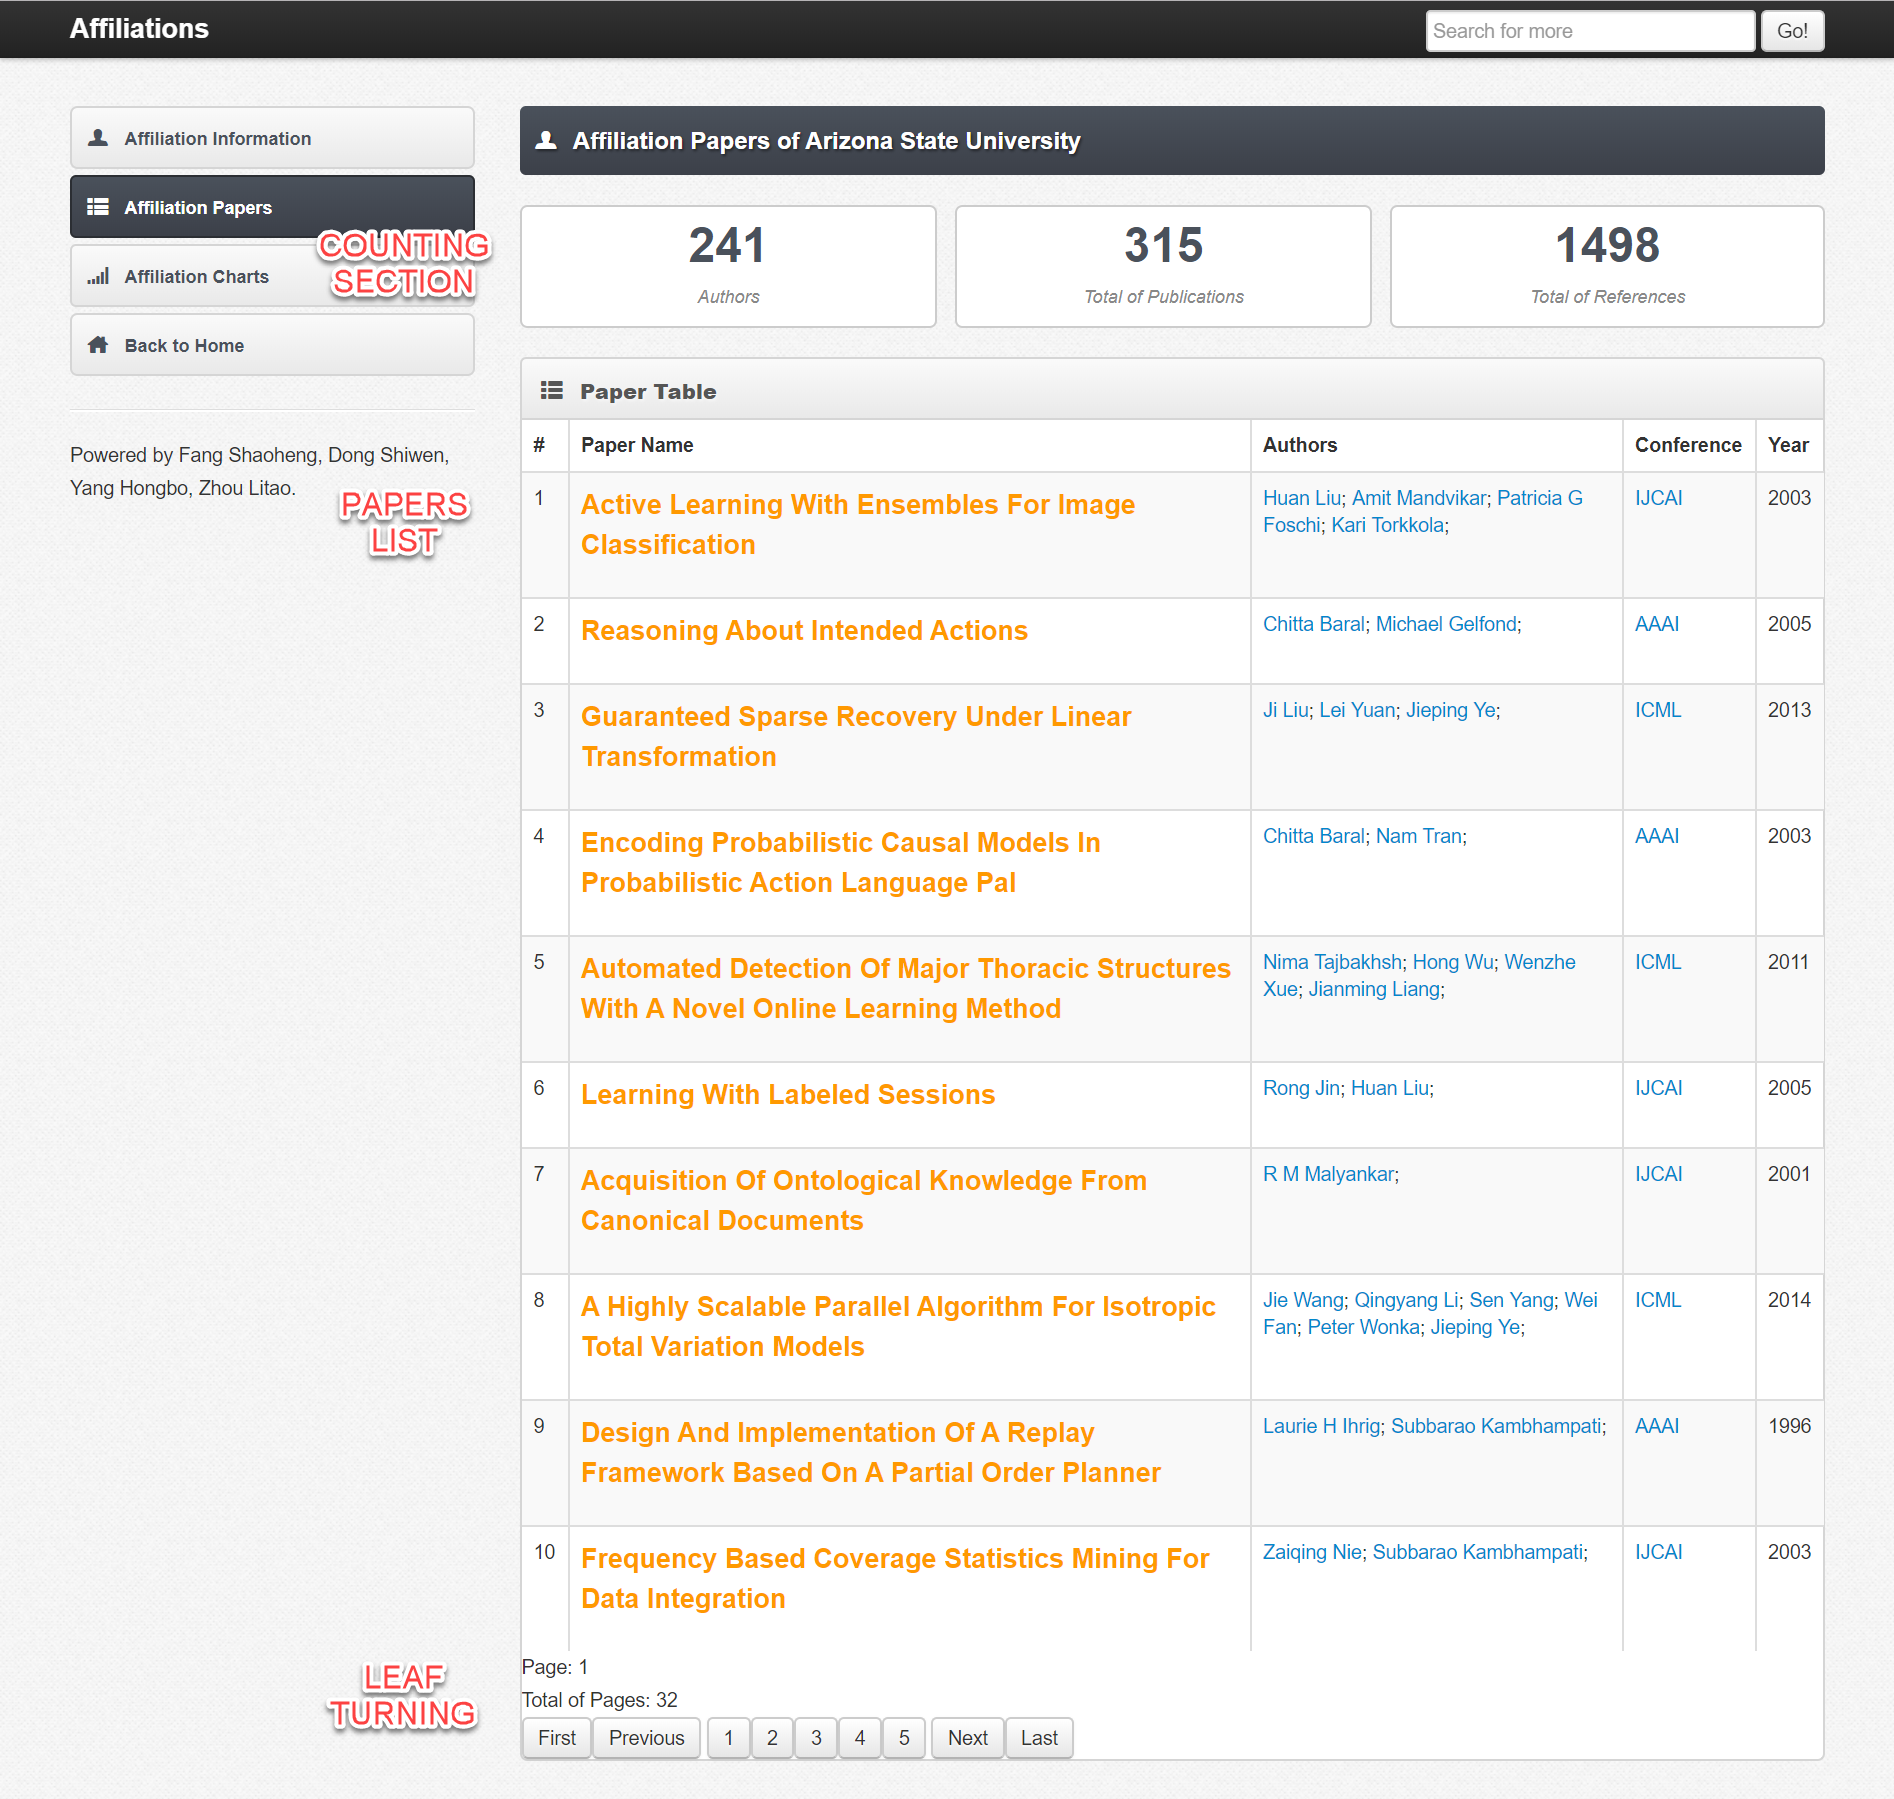
\includegraphics[scale=0.35]{img/zlt_aff_demo2.png}
\caption{affiliation\_paper.php page}
\end{figure}

In fact, for the same function to be displayed on the page, we did two versions of code to implement them. The first one was very basic, just like those in the paper/author/search pages. However, since all the affiliation data are selected from the big paper\_author\_affiliation table, the first version didn't perform well in loading speed. Our optimization will be introduced in the Optimization Chapter.



\subsection {Total Counts}
On top of every affiliation page, we've counted all the authors, papers and references concerned. For authors and papers, we can directly count them in the paper\_author\_affiliation table. For references, we first select the papers and then join the selected results to the paper\_reference table in order to count the results. The MySQL commands are listed below.

\begin{figure}[H]
\centering
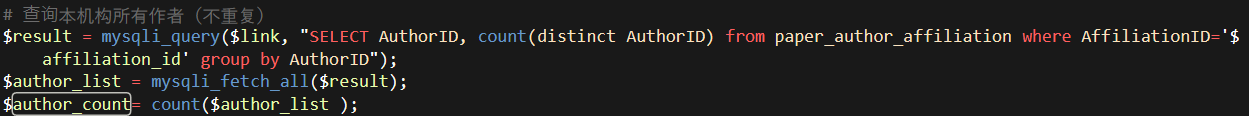
\includegraphics[scale=0.55]{img/zlt_aff_authorcount.png}
\caption{Count Author Commands}
\label{fig:aff_authorcount}
\end{figure}
\begin{figure}[H]
\centering
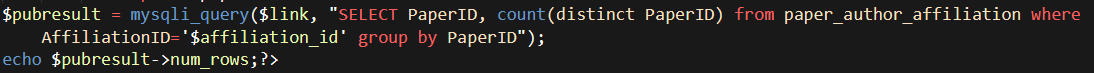
\includegraphics[scale=0.6]{img/zlt_aff_papercount.png}
\caption{Count Paper Commands}
\label{fig:aff_papercount}
\end{figure}
\begin{figure}[H]
\centering
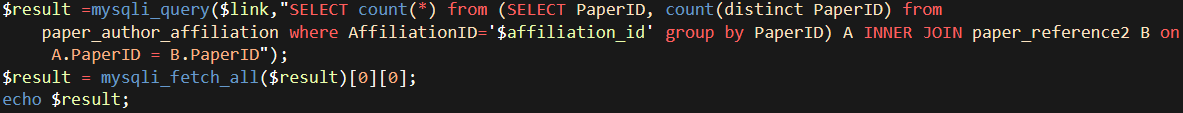
\includegraphics[scale=0.55]{img/zlt_aff_refcount.png}
\caption{Count Reference Commands}
\label{fig:aff_refcount}
\end{figure}

Note that we've use some MySQL techniques such as DISTINCT (eliminate overlapping results) and GROUP BY (perform data counting job) in order to implement our function.

For the data display in our page, our template has already provided a well designed data container in CSS, which can list different numbers in a row, with even width. We can simply apply this pre-defined class in a way demonstrated below.

\begin{figure}[H]
\centering
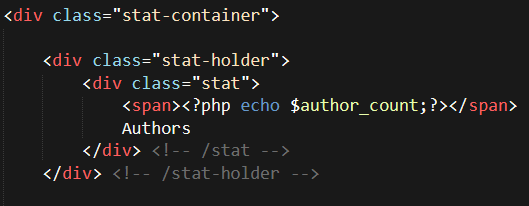
\includegraphics[scale=0.8]{img/zlt_aff_countdisplay.png}
\caption{Use Pre-defined Class to Display Numbers}
\end{figure}


\subsection{Authors List}

The author we've found based on the given affiliaiton may have more than one affiliation where he publishes his paper. So one simple search work is not enough. Luckily, all of the data related to this problem can be selected from the paper\_author\_affiliation table. As a result, our first design is to first sort out all the authors where the affiliation column fits, then we search the table again for affiliation information based on the author's id, which can be realized by looping through the author array in PHP.

In fact, the first step has been done when we count the authors (See Figure \ref{fig:aff_authorcount}), so we simply skip the first step, call the author selecting result in the counting section, and make further searching based on the previous result. During the second step, we've also used DISTINCT \& GROUP BY techniques in order to get the author's affiliation data right and unrepeated.

\begin{figure}[H]
\centering
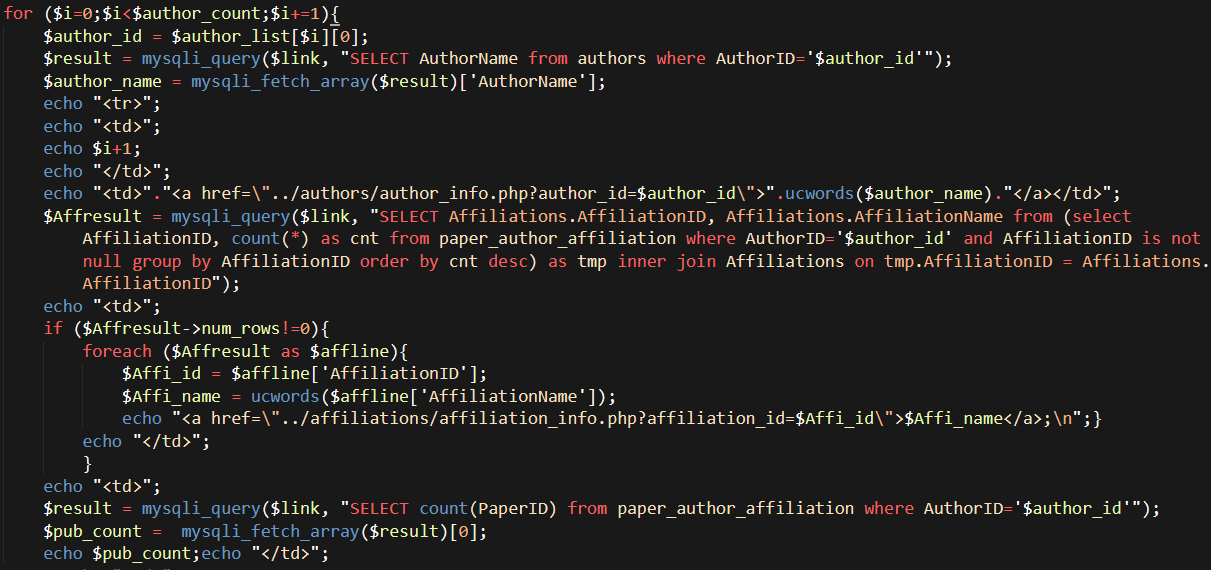
\includegraphics[scale=0.55]{img/zlt_aff_authorloop.png}
\caption{Use Loop to List Author\_Affiliation Information}
\end{figure}

The problem with this solution is that the searching work is too much. Imagine there are 100 authors related to one affiliation, we have to go through the big paper\_author\_affiliation table 100 times in order to get all the data. It turned out that it would take the webpage about half a minute to get completed loaded. The optimization work will be introduced in the Optimization Chapter.

\subsection{Papers List}

The general structure of this list is simlilar to those in citation/ reference/ author's paper list. We may just use MySQL to select all the paper's id related to the affiliation, keep this array storing the paperid we want to display, and the leave the rest of the work to the codes we've already written in the previous work. The selecting MySQL commands are listed below. Actually, just like the case in the author list section, the first step has also been completed in the counting section. (See Figure \ref{fig:aff_papercount}) So there are no codes left for this section to explain.

\chapter{Leaf Turning}

dsw

\section{Version I: by PHP parameters}

\subsection{Description}

\subsection{Solution}

\paragraph{point 1}

\paragraph{point 2}

\subsection{Source Codes}

\begin{minipage}[r]{15em}
\begin{verbatim}

short code example

\end{verbatim}
\end{minipage}

\subsection{Explanation}

\subsection{Demonstration}

\begin{figure}[H]
\centering

\includegraphics[height=4.0cm,width=4.0cm]{img/dsw_1.jpg}
\caption{IMG EXAMPLE}
\end{figure}


\section{Version II: by jQuery}



\chapter {Integrated Searching Bar}

fsh


\chapter {Data Visualization}


\section {Statistical Graph}

fsh

\subsection{Description}

\subsection{Solution}

\paragraph{point 1}

\paragraph{point 2}

\subsection{Source Codes}

\begin{minipage}[r]{15em}
\begin{verbatim}

short code example

\end{verbatim}
\end{minipage}

\subsection{Explanation}

\subsection{Demonstration}

\begin{figure}[H]
\centering

\includegraphics[height=4.0cm,width=4.0cm]{img/fsh_1.jpg}
\caption{IMG EXAMPLE}
\end{figure}



\section {Paper Relation Graph}

A relation graph can visually reveal the relationship between papers, which we believe will be of great help to the users. For every paper, we've prepared a relation graph to show its reference papers, and the reference papers of its reference papers. Visitors can have a clear picture of how the paper is derived by looking at multiple levels of reference papers.

\subsection{Description}

We've applied a built-in template in echarts when making the relation graph. First we've fetched all the paper\_reference relationship concerned, including multiple levels of reference relations, from the database. Then based on these data, we translate them into two arrays, namely nodes and links, which can be accepted by the echarts template. In the meantime, we add more information such as paper title, weight of the nodes and styles of the links into the array. Then the relation chart can be generated by echarts. In addition, we also wrote a jQuery function by ourselves in order to allow our users to visit the cited paper directly by clicking the nodes or the links. Some demo screenshots are listed below.

\begin{figure}[H]
\centering
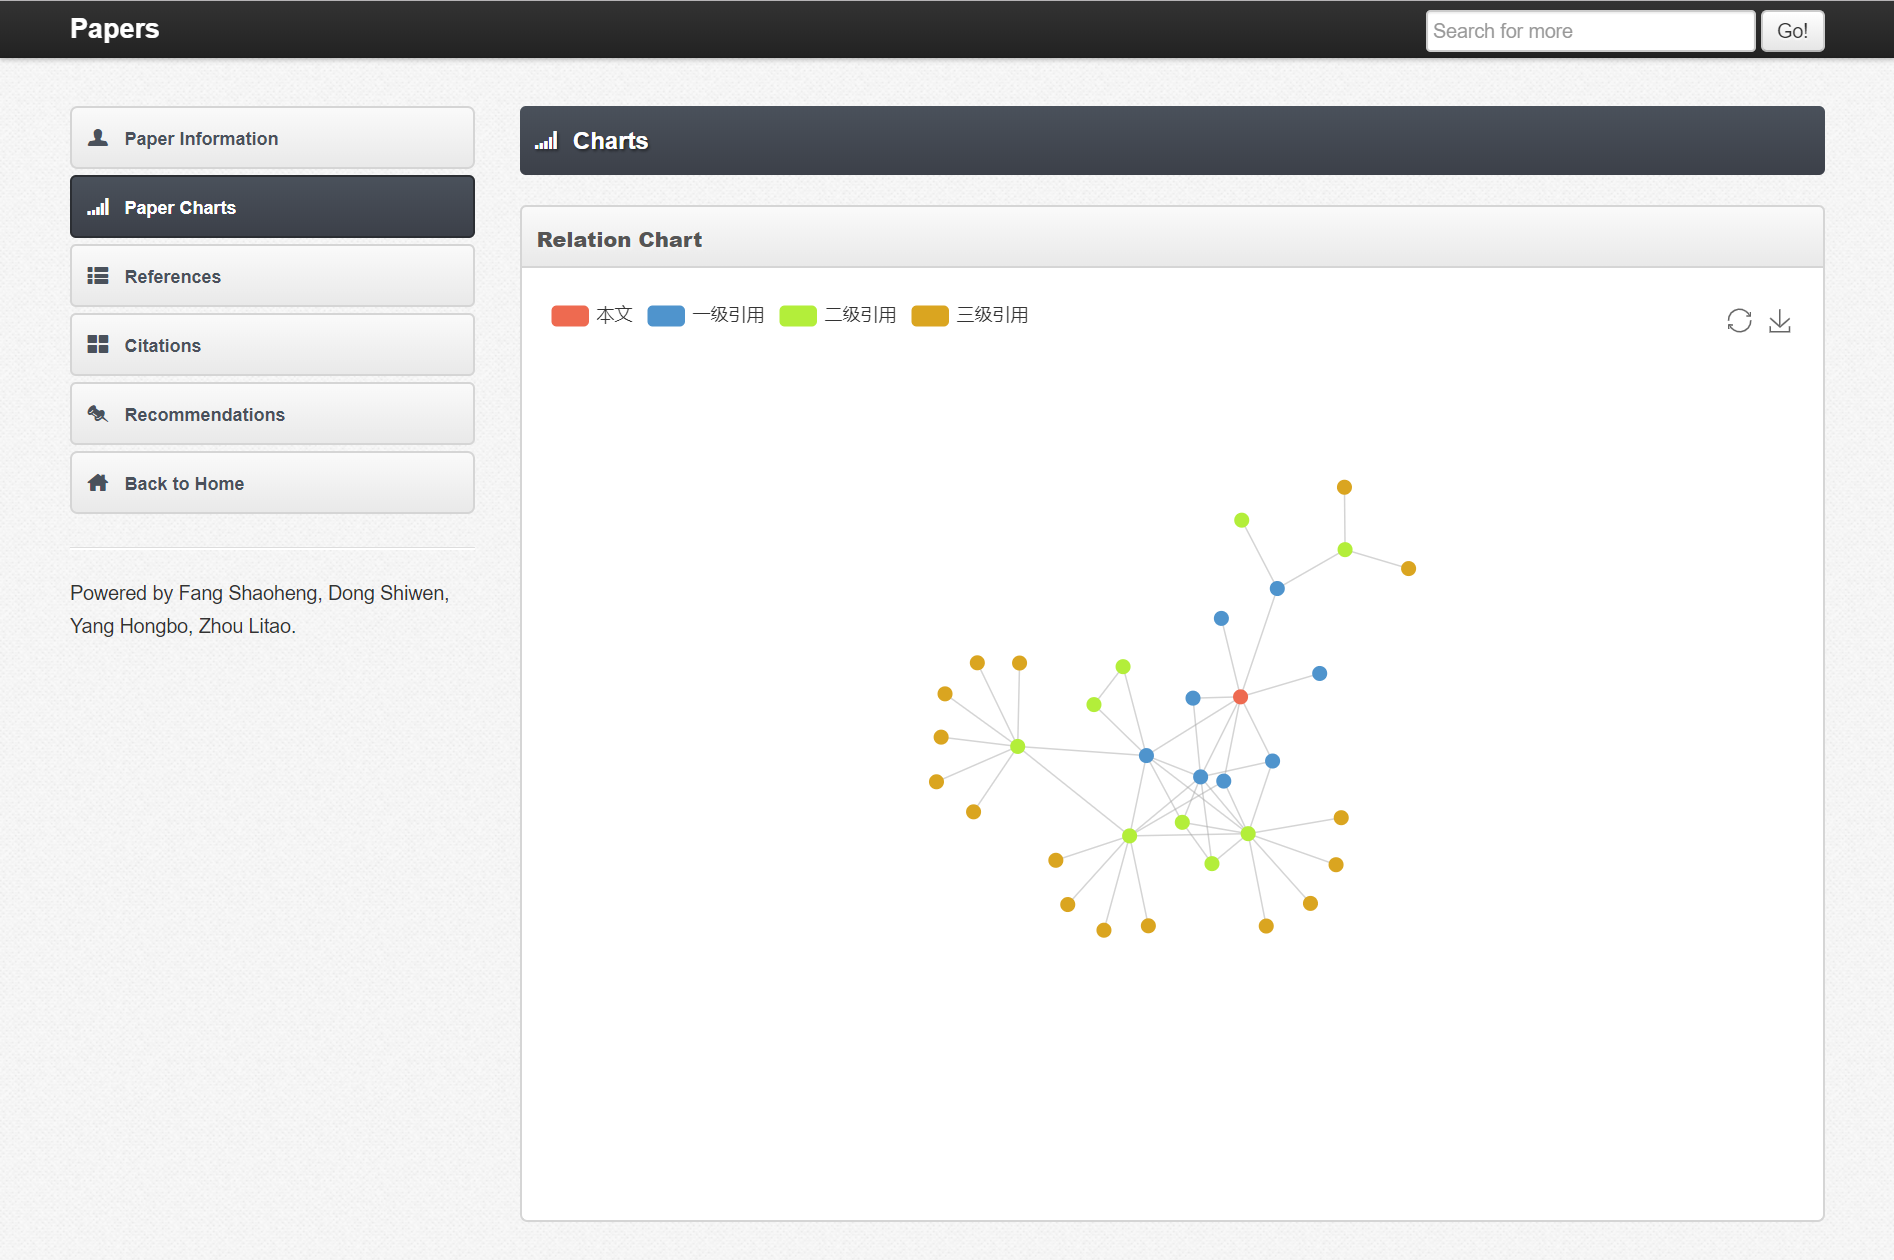
\includegraphics[scale=0.4]{img/zlt_rel_demo.png}
\caption{Relation Chart Page}
\end{figure}

\begin{figure}[H]
\centering
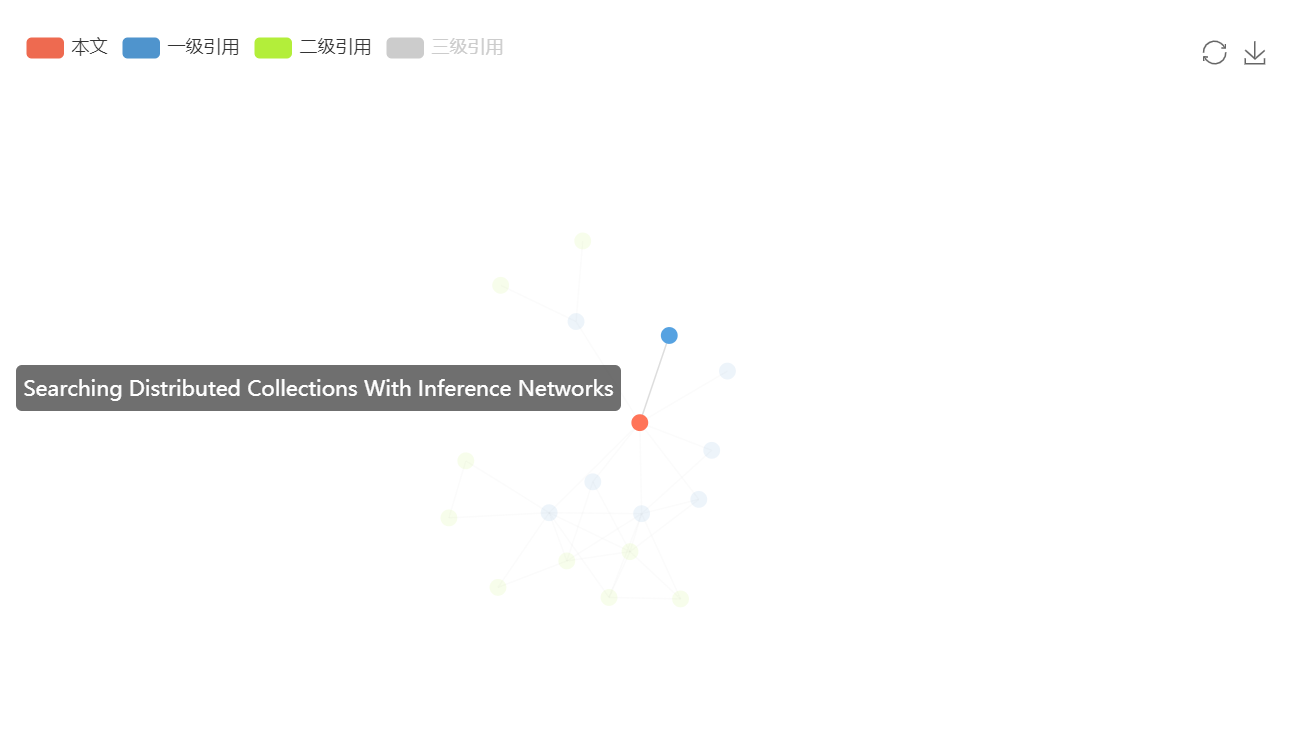
\includegraphics[scale=0.3]{img/zlt_rel_demo1.png}
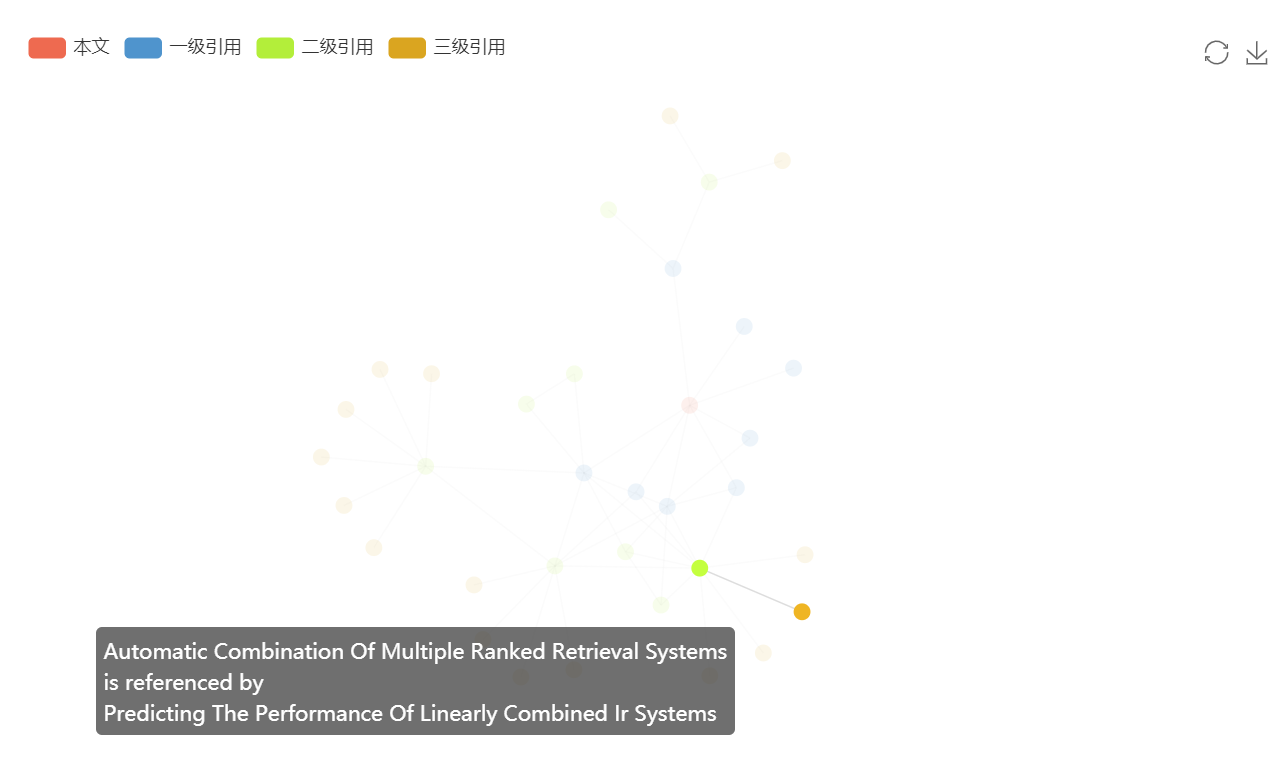
\includegraphics[scale=0.3]{img/zlt_rel_demo2.png}
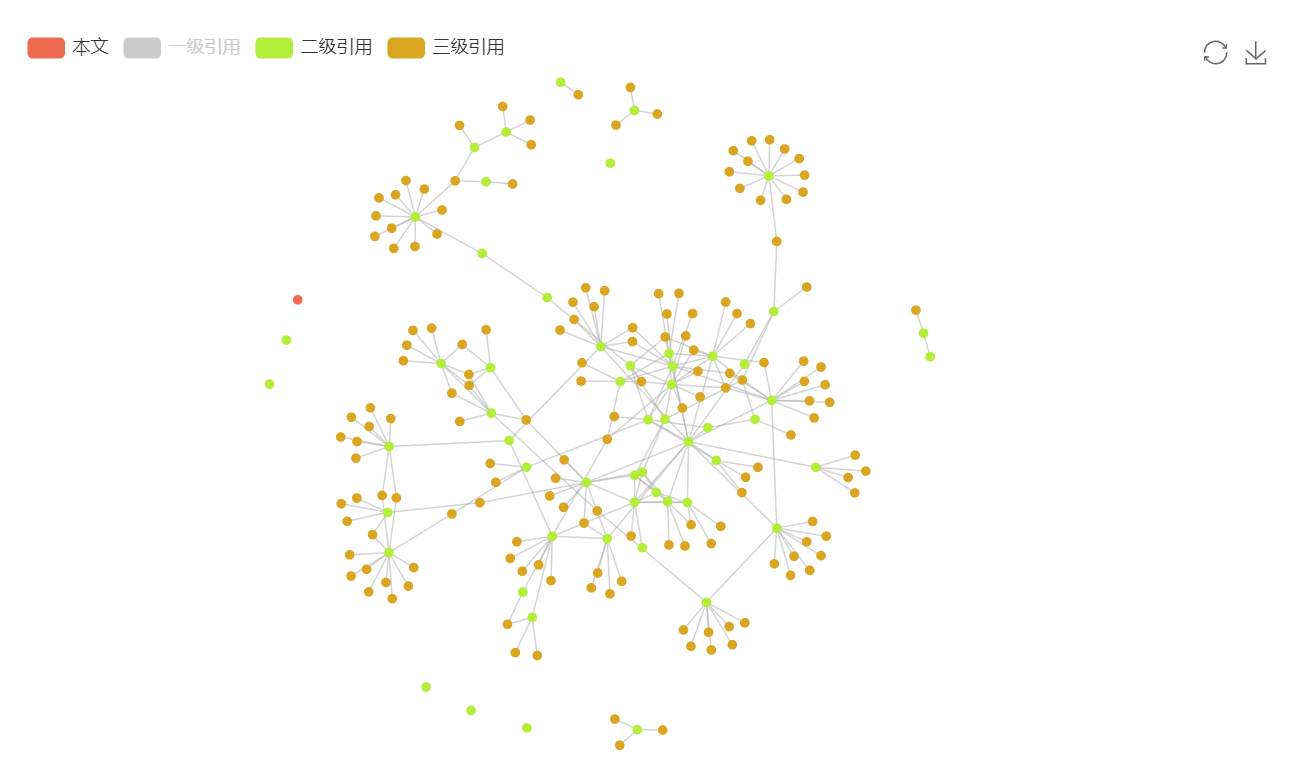
\includegraphics[scale=0.3]{img/zlt_rel_demo3.png}
\caption{Multiple Display Modes \& functions}
\end{figure}

\subsection{Collect the Data}

For convenience's sake, we first wrote a function in order to integrate the search of a paper's name into a function call. The ucwords() is a useful function in PHP, which can turn the first letter of every word into upper case. This can give our information display a better look.

\begin{figure}[H]
\centering
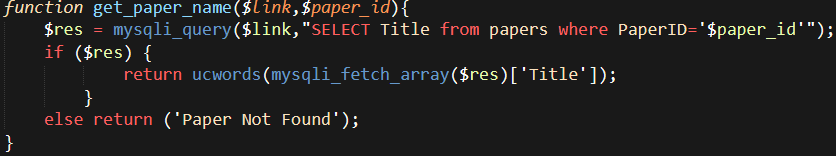
\includegraphics[scale=0.55]{img/zlt_rel_code_func.png}
\caption{get\_paper\_name function}
\end{figure}

Then we use MySQL to get the direct reference of the paper. For these referenceIDs, we wrote a loop to add them to the nodes array, and put these first-level relations directly into the links array.

\begin{figure}[H]
\centering
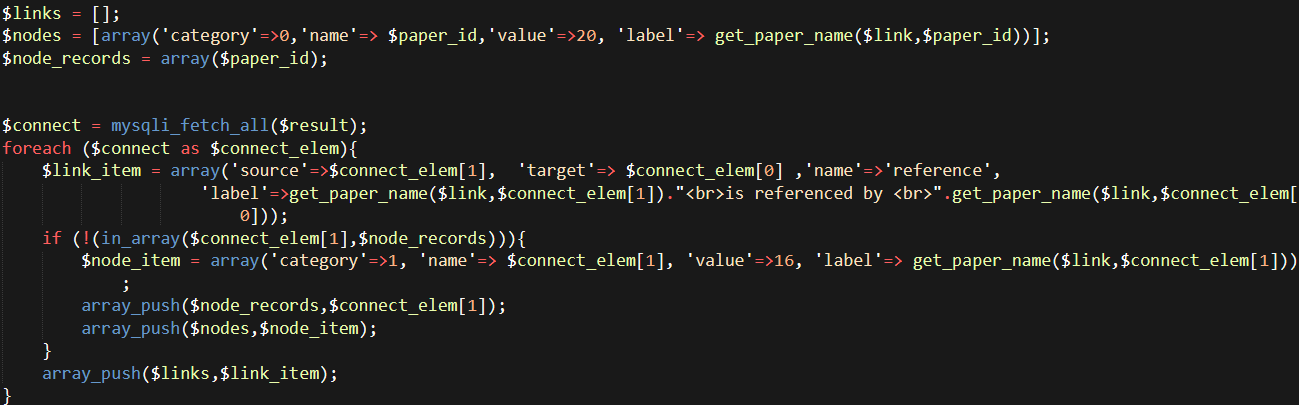
\includegraphics[scale=0.55]{img/zlt_rel_code_lev1.png}
\caption{First Level Data Collection}
\end{figure}

After that, we wrote a nested loop. The first level is to loop through the depth (i.e. the reference level), the second level is to loop through reference papers of the last reference item. The searching structure is just like building a tree. Note that we've created a helping array storing the paperids that we've already added into the nodes array, so that we can avoid overlapping nodes. Theoretically, the reference level (depth) can be streatched to infinity, but for practical use, we assume the depth of 4 will be fine.

\begin{figure}[H]
\centering
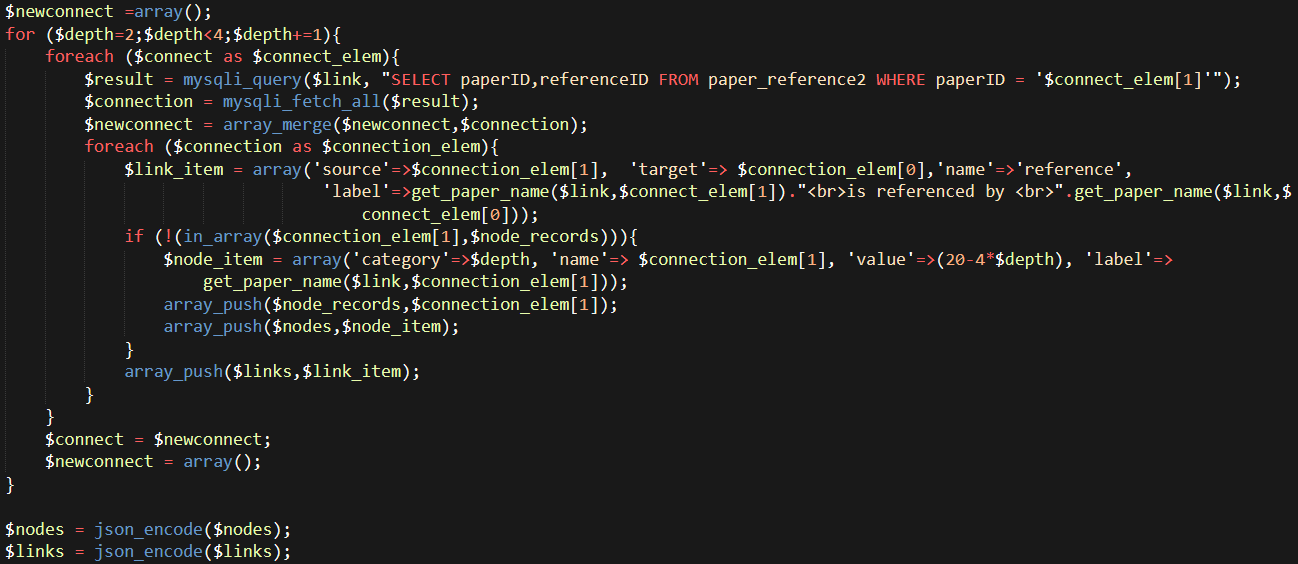
\includegraphics[scale=0.55]{img/zlt_rel_code_lev2.png}
\caption{Higher-Level Data Collection}
\end{figure}


\subsection{Set Echarts Options}

The links and nodes arrays we've created above are just what the built-in echarts template requires. However, the initial graph configurations were not suitable for our information. (See Figure \ref{fig:rel_contrast}) We need to block the display of node ids and loosen the distance between dinstinct nodes. After some manual regulating work, we make the graph look a lot better. Our major configuration codes are listed below.

\begin{figure}[H]
\centering
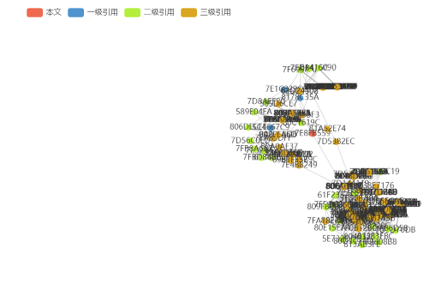
\includegraphics[scale=0.55]{img/zlt_rel_demo4.png}
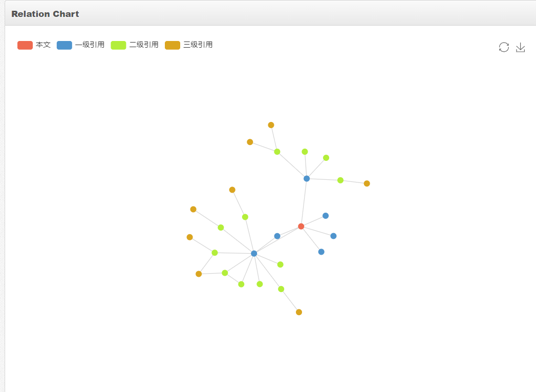
\includegraphics[scale=0.55]{img/zlt_rel_demo5.png}
\caption{A Contrast between the Original and the Present Version of Paper Relation Charts}
\label{fig:rel_contrast}
\end{figure}

\begin{figure}[H]
\centering
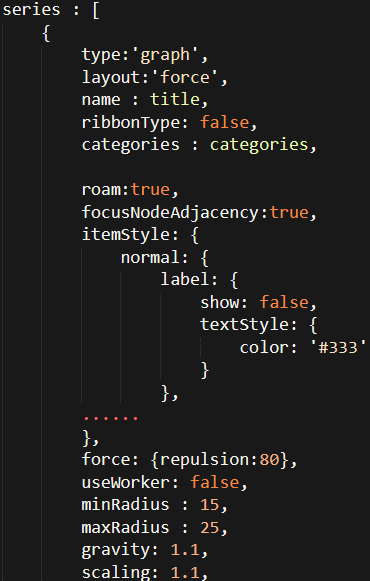
\includegraphics[scale=0.55]{img/zlt_rel_code_config.png}
\caption{Echarts Options Configuration}
\end{figure}

\subsection{Node Labels}

The labels of our nodes should show the paper's name and the labels of our links should show the name of the two papers in the reference relation. This work has already been finished when we are collecting the data. We set the label of the nodes to be exactly what we want to show to our users. A further step we took is to add hyper-links to every nodes and edges. Note that the name of every node is its PaperID, which can be directly applied to the URL, while the name of every link is composed of the reference node and the origin node. We use the string carving function in PHP to get the first 8 character, representing the reference node, so users can access the reference page by clicking the links.

\begin{figure}[H]
\centering
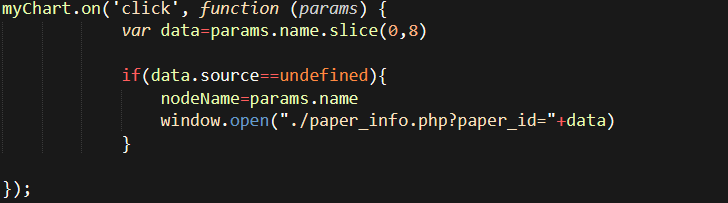
\includegraphics[scale=0.55]{img/zlt_rel_code_label.png}
\caption{Create Hyper-links for Node Labels}
\end{figure}


\section{Big Charts using Gephi}

As the saying goes, ``One picture worths 1000 words.'', a visualization picture is vital to show the connection between objects in some scales. To show an overall relationship, we choose  \textbf{gephi} to visualize the data collected by MySQL. This method can help the part of E-charts to draw a better pictue in users' mind. 
There was a problem that troubled us for a long time. That is: how can we put the picture onto the pages. And it is finally solved by using package ``ariutta/svg-pan-zoom
'' from GitHub. 
Here we'll give MySQL sequences and the way to draw a gephi picture(.svg).

\subsection{MySQL Fetch}

We choose to show the connection between authors in all 13 conferences. We established the connection by reference and citation. And this demands us to use `join search' in MySQL. Example codes are given below.(We take ConferenceID= `47c39427' for an example.)

\begin{figure}[H]
\centering

\includegraphics[height=4.0cm,width=18cm]{img/yhb_my_1.png}
\caption{search example}
\end{figure}

Finally, remember to lead the data out in (.csv) format, in order that we can use the data in gephi easily.

\subsection{Gephi Drawing}

Gephi can use data in (.csv) format directly. After transmitting information into gephi, we can find a picture in the window. But this picture is so ugly and unclear that we cannot take it for visualization use derectly.  

\begin{figure}[H]
\centering

\includegraphics[height=7.0cm,width=18.0cm]{img/yhb_ge_1.png}
\caption{geghi: original picture}
\end{figure}
We may turn to gragh-drawing methods such as ``force directed method'' and ``Fruchterman Reingold method'', to better display the characteristics of the relationship between authors.

Next, we can adjust the  size of each node by degree, and give them different colors.
It's much easier for us to see the relation.
\begin{figure}[H]
\centering
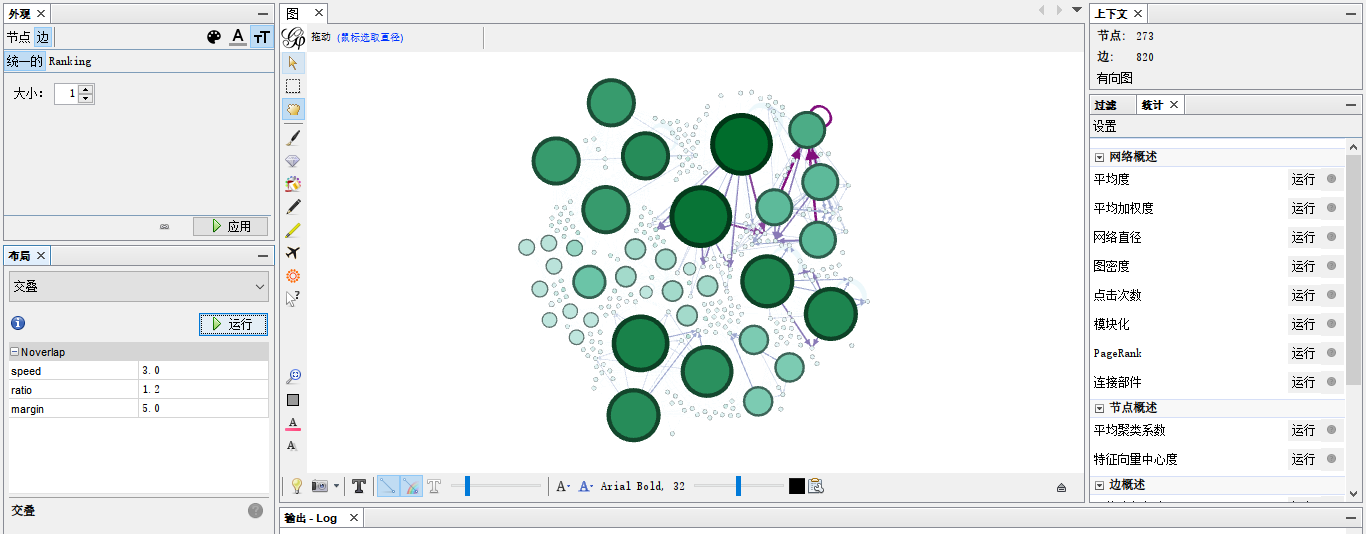
\includegraphics[height=7.0cm,width=18.0cm]{img/yhb_ge_2.png}
\caption{geghi: processed picture}
\end{figure}
Finally, we can transmit it as (.svg) file to load on the pages.

\chapter {Beautify the Pages}

\section {Index Beautification}

fsh

\section {Pages Beautification}

Our original page styles were derived from LAB3, which were very basic. With more and more functions implemented, we found that one page was not enough to carry all the information. As a result, we decided to split one page into several subpages carrying out different functions. For example, we split the paper.php page into information page, charts page, reference page, citation page and recommendation page. With the help of online resources, we fit our contents into a well-defined template. (tribute to http://www.cssmoban.com)


\begin{figure}[H]
\centering{}
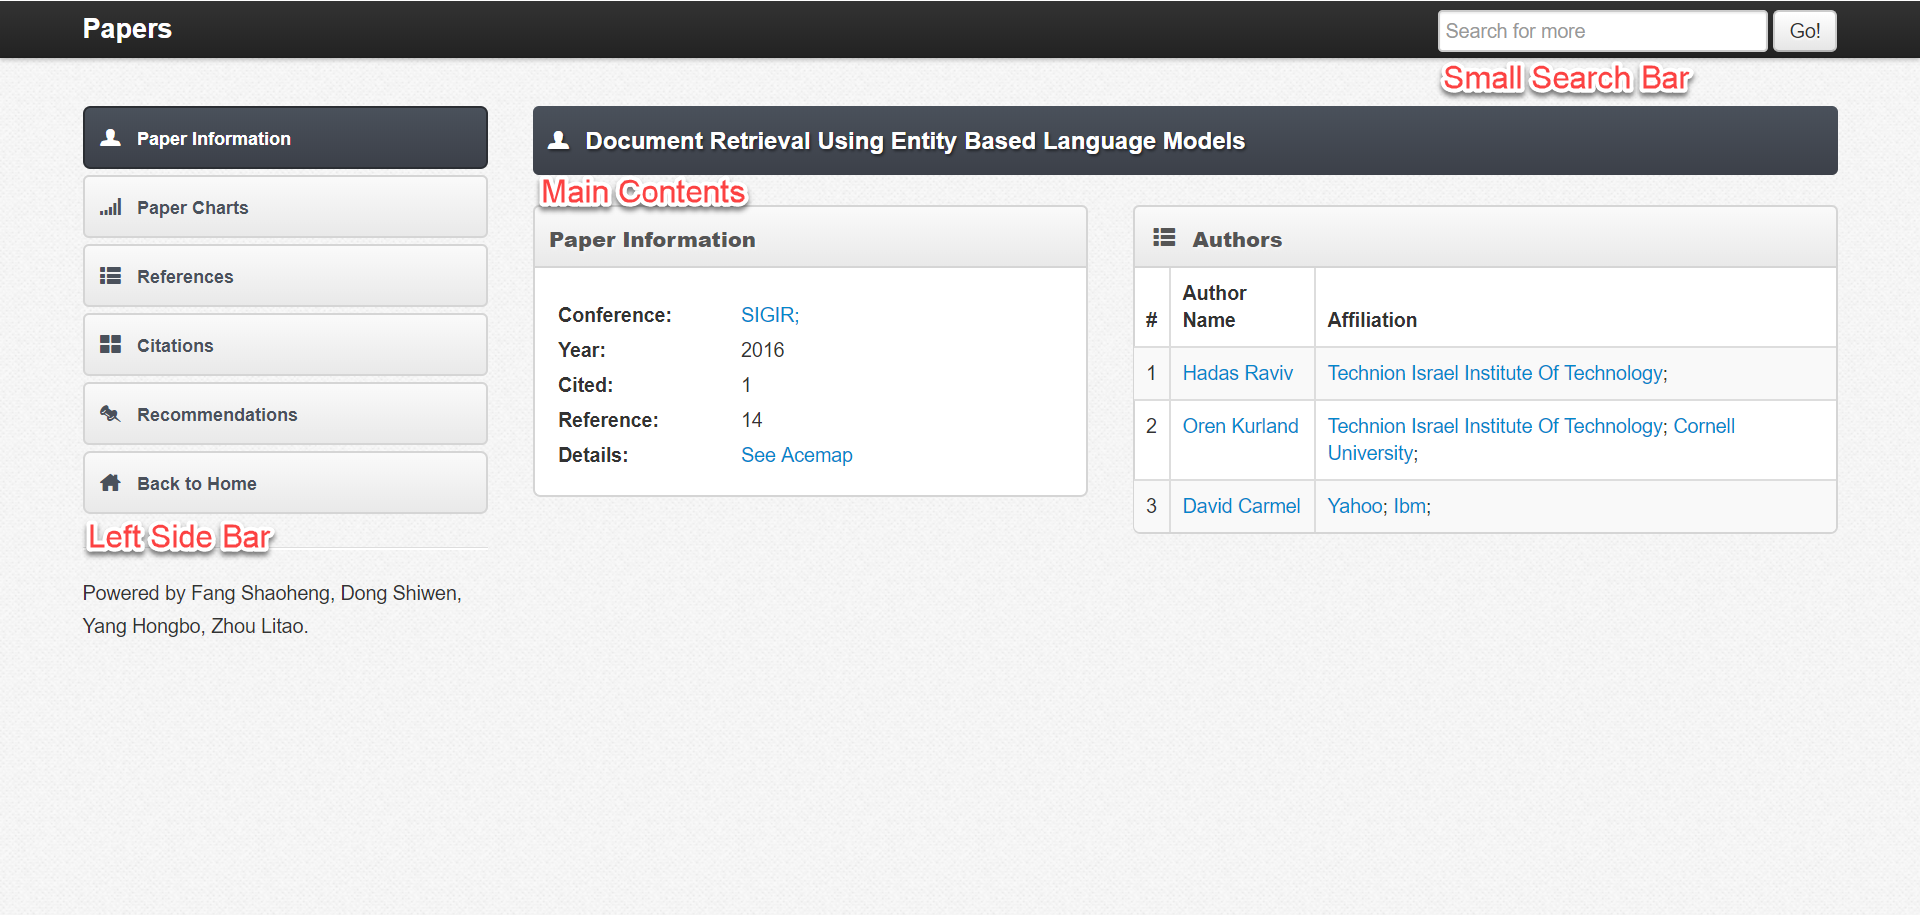
\includegraphics[scale=0.35]{img/zlt_beau_demo.png}
\caption{General Structure of the Pages}
\end{figure}

As the screenshot above reveals, all the pages share a similar layout - a top banner containing the page title and a small search bar, a right navigating column linked to all the related pages in this section and the right division where the main contents of the page are located.

\subsection {Top Banner \& Small Search Bar}

Our template was originally designed for backstage admin system. In order to better fit our webpages, we replace the user login button with a small search bar. The search bar was a simple <form> application, but it turned out to be very useful when we are testing and using our pages. Codes of this part are listed as follows.

\begin{figure}[H]
\centering{}
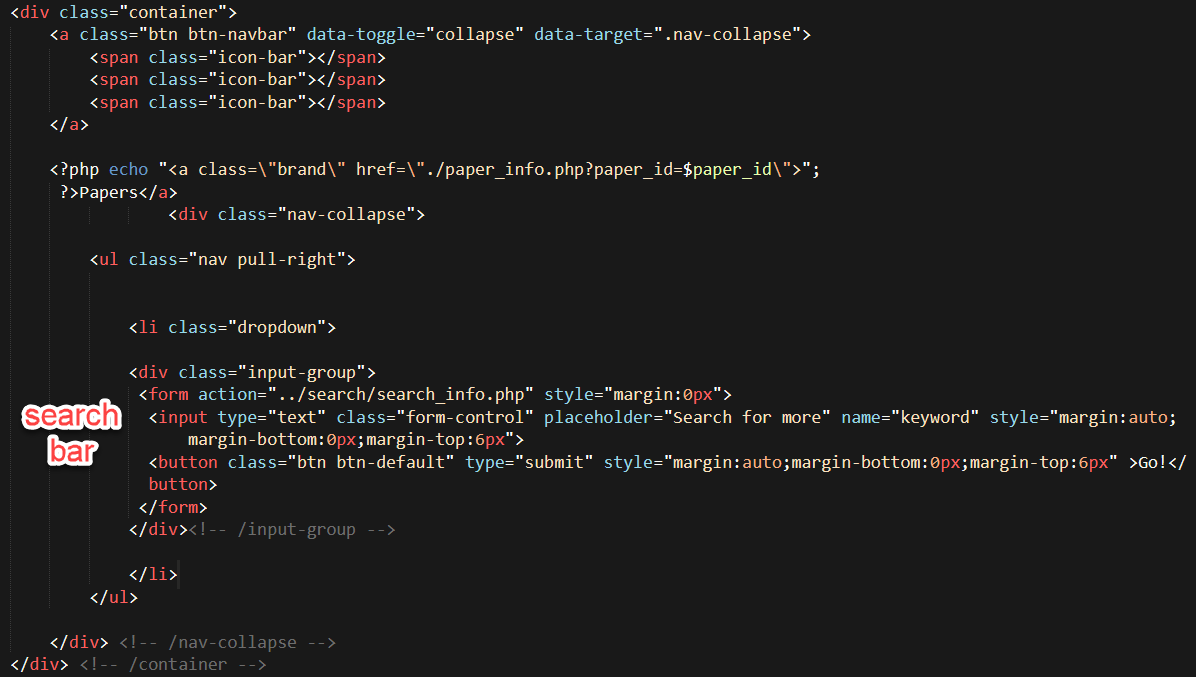
\includegraphics[scale=0.35]{img/zlt_beau_codes.png}
\caption{Top Banner}
\end{figure}


\subsection {Left Navigation Bar}

The template has already provided a series of button icons (derived from bootstrap framework) and a well-formatted list of buttons. To make our own navigation bar, we just need to change the icons according to the given names, and get the name and hyper-links right. Also, we can specify the class to be ``active'' in order to highlighten the button representing the current page.

\begin{figure}[H]
\centering{}
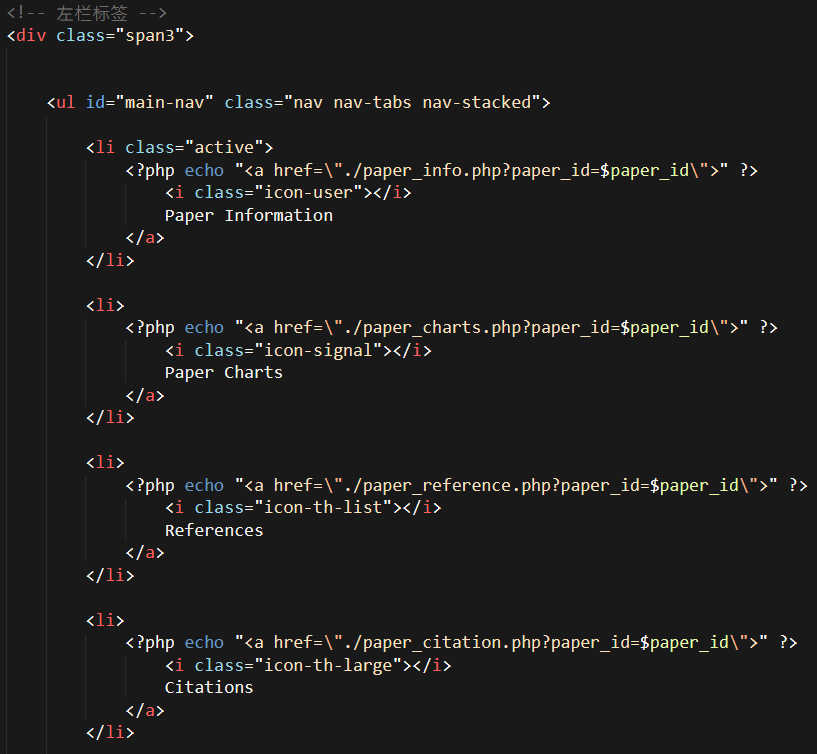
\includegraphics[scale=0.35]{img/zlt_beau_bar1.png}
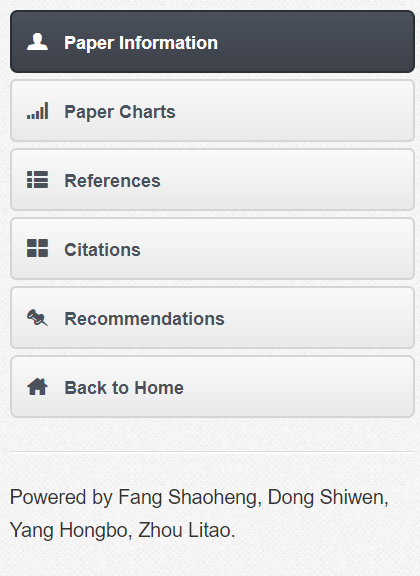
\includegraphics[scale=0.35]{img/zlt_beau_bar2.png}
\caption{Left Navigation Bar}
\end{figure}

\subsection {Main Contents}

Since the template is based on the framework of Bootstrap, in the main contents, it follows that we should obey the rules of Bootstrap, such as containers, row classes, and the twelve column layout. Take a particular page for example, the generating process of the table through PHP is omitted. The layout for other pages are simlar in principle.
\begin{figure}[H]
\centering{}
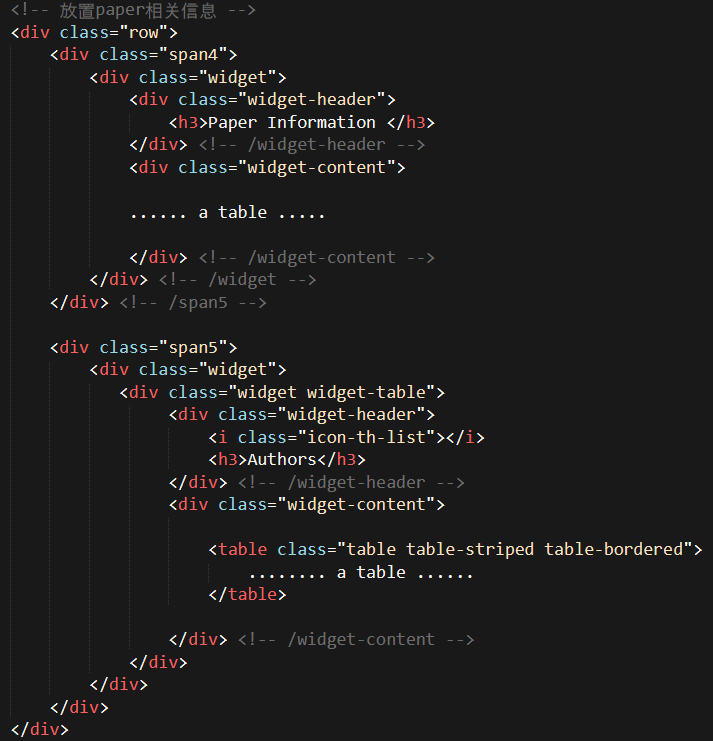
\includegraphics[scale=0.35]{img/zlt_beau_cont1.png}
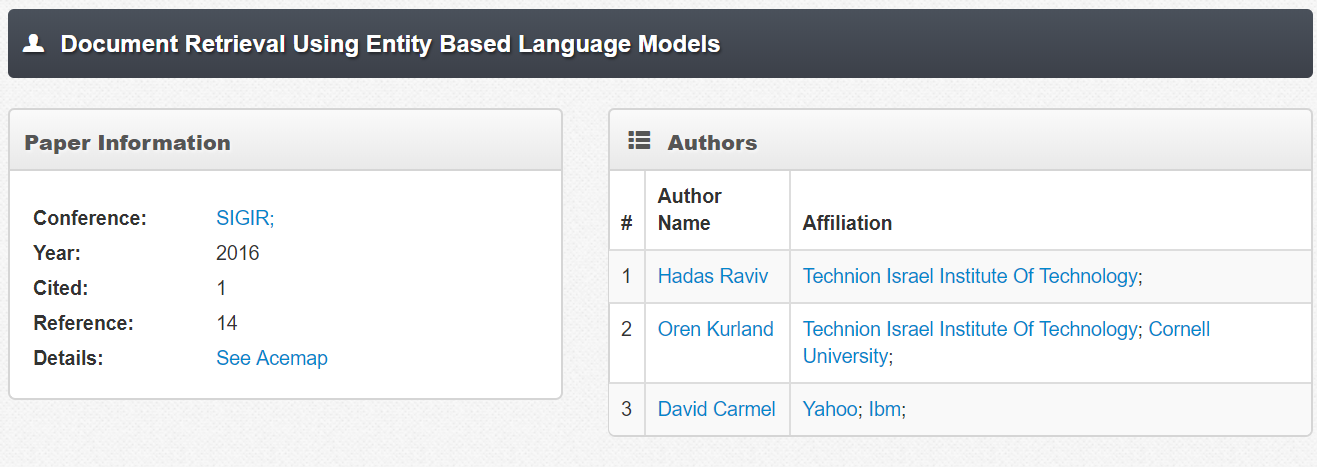
\includegraphics[scale=0.35]{img/zlt_beau_cont2.png}
\caption{Main Contents}
\end{figure}



\chapter {MySQL Optimization in Affiliation Pages}

The affiliation section is a section all made by ourselves. However, as has been briefly introduced in the Affiliation Pages section, new problems arise that the loading speed is too slow. This is because in our solution, the big paper\_author\_affiliation table will be searched everytime we display a new row in the webpage, which is clearly unnecessary. (See Figure \ref{fig:opt_basic})
{}
\begin{figure}[H]
\centering{}
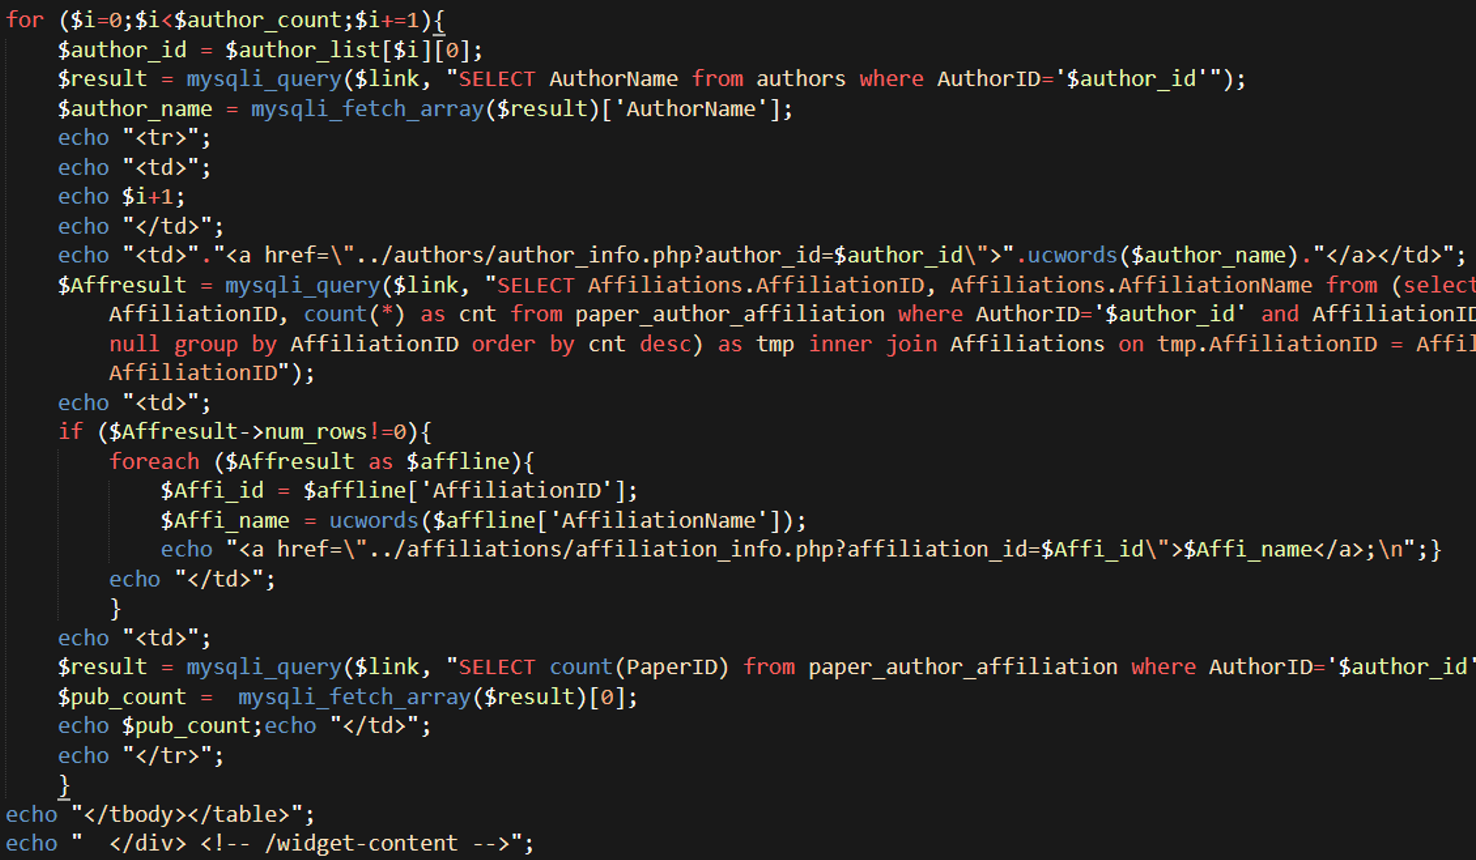
\includegraphics[scale=0.45]{img/zlt_opt_code_basic.png}
\caption{Base Version in Affiliation Pages}
\label{fig:opt_basic}
\end{figure}


\section {Solution}
Through practice, we found that the main factor dragging the loading time slow is the call by PHP for MySQL query. In order to reduce the loading time, we need to control the time we call a MySQL query. However, generally speaking, since we first need to get the authors based on the affiliation\_id, and then find the detail information based on the author we have found in the first query, there is an unavoidable iterating structure in the process. The solution to this problem is not as easy as we assumed.

Eventually, we came up with the idea that all the searching work with MySQL can be integrated into one query. And we may just select the information we need from the total query results in order to display the information in the pages. This solution has restricted the searching query call to one single time. However, this will creat some difficulty when we want to echo the information onto the webpage.

\section {Integrated MySQL Query in Authors List}

Instead of searching the author information piece by piece, the searching query we write (See Figure \ref{fig:opt_query}) will return a group of rows showing the paper / affiliation information about one single author.

The basic idea about this integrated query is join the paper\_author\_affiliation table to itself, with restricting conditions of course. Our final result is a simplified paper\_author\_affiliation table, containing the author directly linked to the affiliaiton and the papers which might not be published in this affiliation, but whose authors once belonged to the affiliation. With the GROUP BY technique, the rows of every author can be returned group by group.

\begin{figure}[H]
\centering
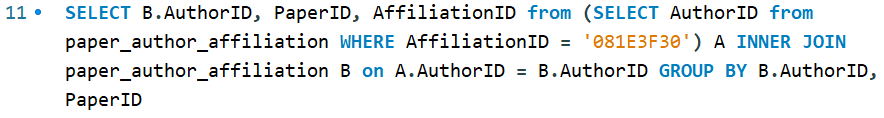
\includegraphics[scale=0.55]{img/zlt_opt_code_query.png}
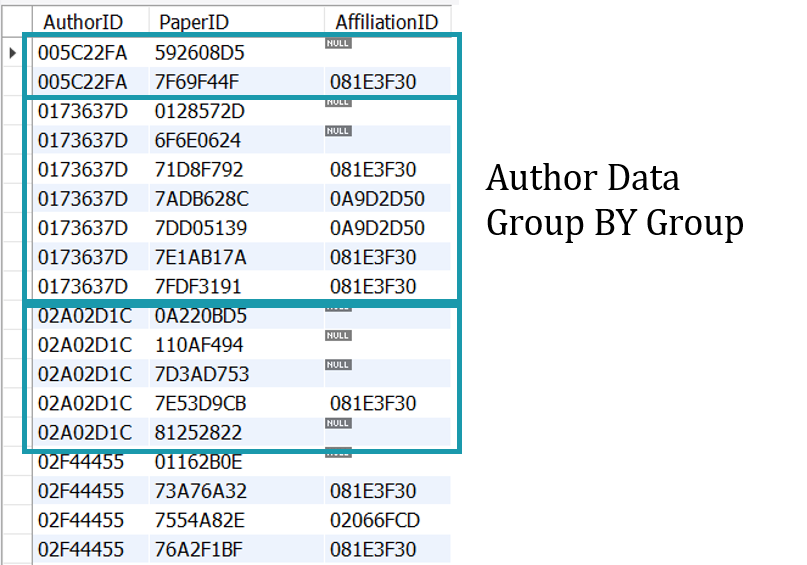
\includegraphics[scale=0.55]{img/zlt_opt_code_queryres.png}
\caption{Integrated MySQL Query}
\label{fig:opt_query}
\end{figure}

\section{Echoing Tricks in Authors List}

Unlike what we did in the base version, where MySQL queries and PHP iterative loops are mixed together in an intuitive structure, here we are looping through the rows in the integrated searching results. (See Figure \ref{fig:opt_query}) So in every loop, we need to first judge whether this row is talking about the same author above or it starts a new one. Within the group corresponding to the same author, we just add one more affiliation into the webpage (before that we have to judge whether the affiliation is a new one, of course). While if the row marked the start of a new author, we have to end the previous row, begin a new row on the webpage. With these tricks, the final outlook on the webpage is just the same as the base version, but boasts a loading time within a second. The main part of the codes are listed below. (Initialization and Clean-up work omitted) The same tricks also apply to Paper List on the affiliation\_paper page. 


\begin{figure}[H]
\centering{}
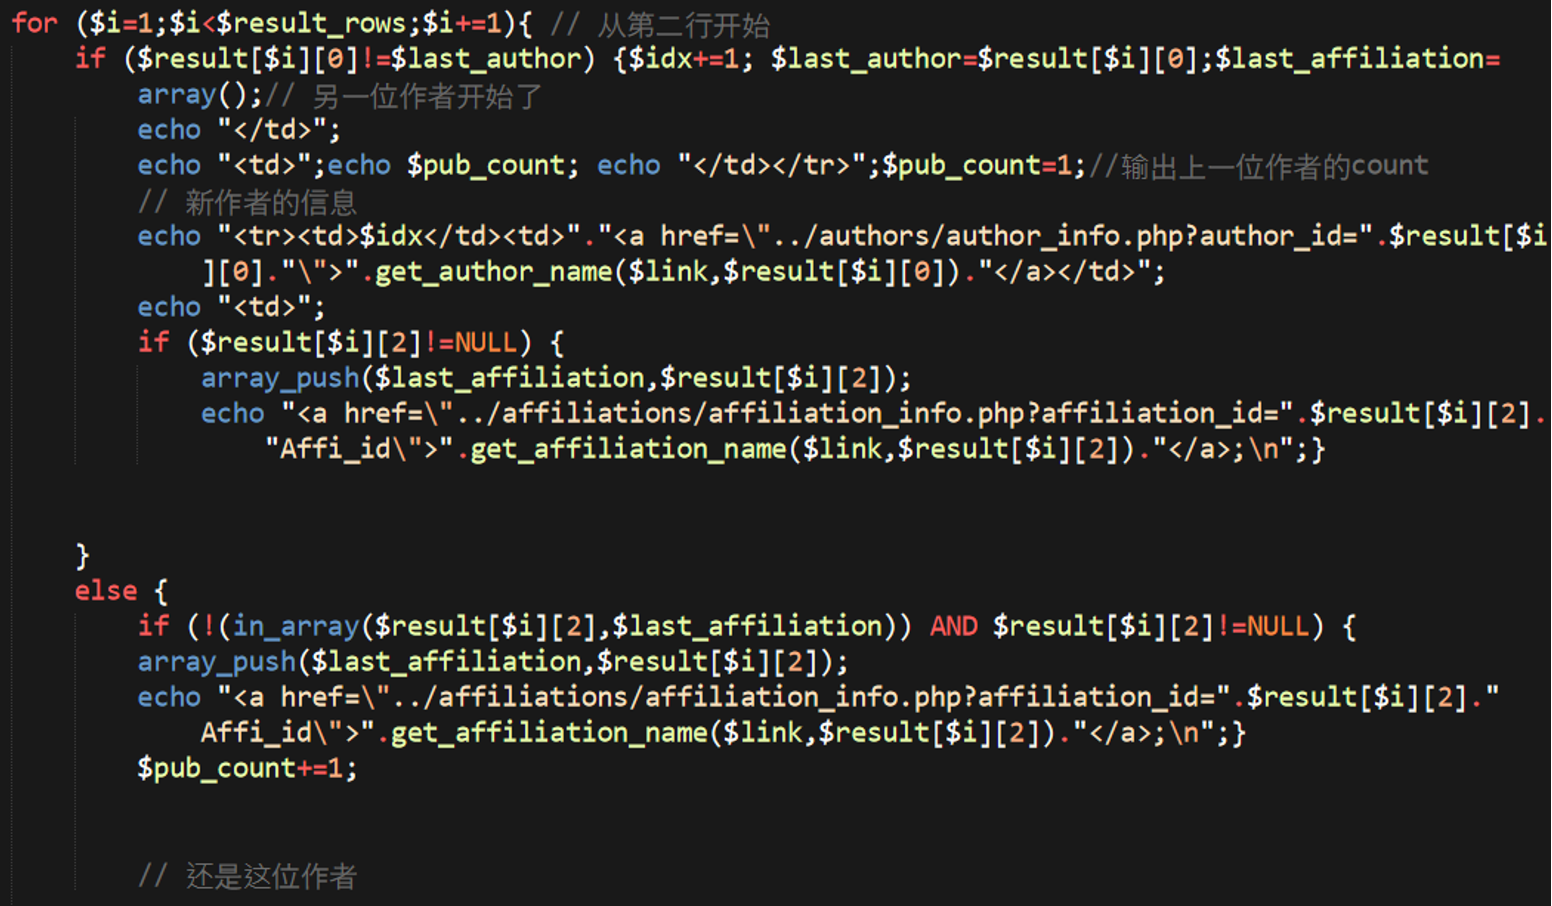
\includegraphics[scale=0.45]{img/zlt_opt_code_advanced.png}
\caption{Echoing Tricks}
\end{figure}

\section{Integrated MySQL Query in Top Authors Charts}

As has been discussed before in the Charts section, the top author charts require a list of author names and a list of numbers representing their publications counts. The same problem occurs that the data collecting work was taking too much time. We are also using MySQL joint search to replace PHP loops. We use count (DISTINCT ) + GROUP BY commands to directly get the result. The MySQL queries are listed below. Further processing on the searching results are fragile and hence omitted. 

\begin{figure}[H]
\centering{}
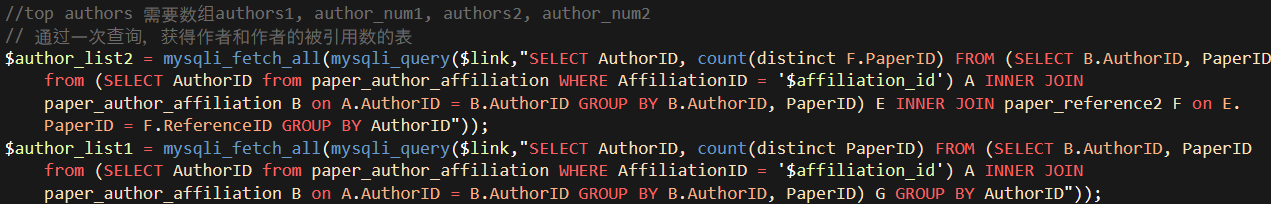
\includegraphics[scale=0.55]{img/zlt_opt_code_chart.png}
\caption{Integrated MySQL Query in Top Authors Charts}
\end{figure}

All the three parts introduced above make up our optimization of the affiliation section.

\end{document}
